\documentclass[fontsize=20pt]{scrartcl}
\usepackage[margin=0.5in, a4paper, landscape]{geometry}
\usepackage{tikz}
\usepackage{amsmath}
\usepackage{pgfplots}
\usepackage{siunitx}
\usetikzlibrary{calc,patterns,angles,quotes}
\begin{document}
Reflect the vector in the line $y=x$:
\newline
\newline
\begin{tabular}{p{13cm}p{13cm}}
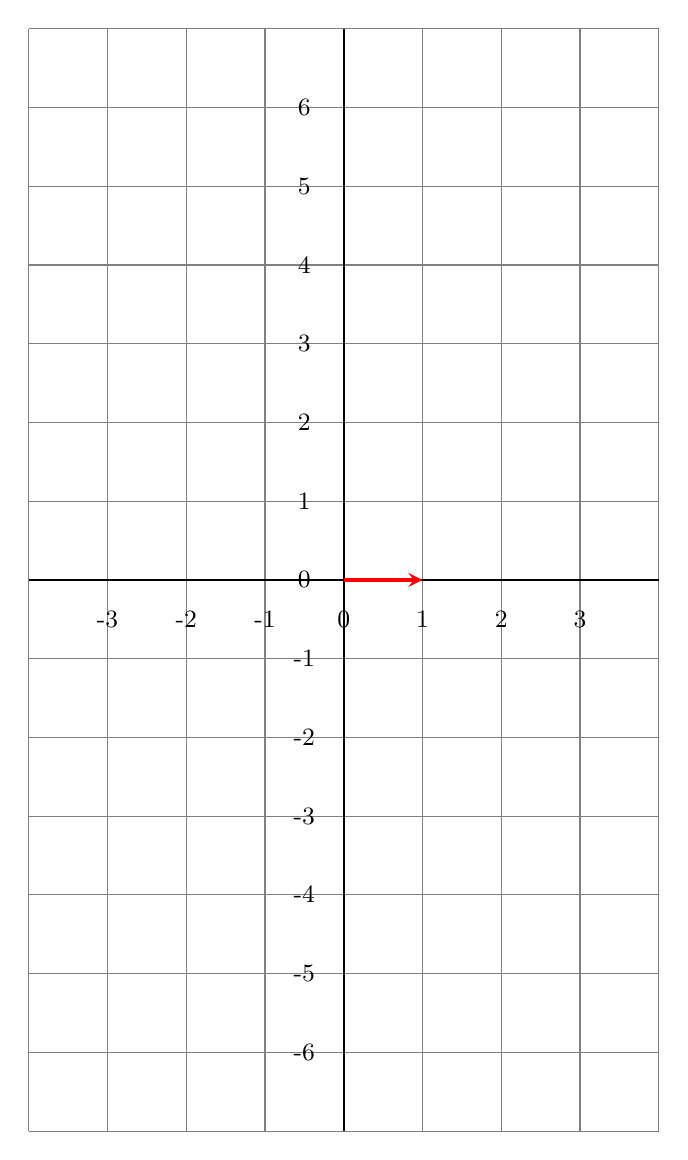
\begin{tikzpicture}
\draw[thin, step=1cm,color=gray] (-4,-7) grid (4,7);
\draw[thick] (-4,0)--(4,0);
\draw[thick] (0,7)--(0,-7);
\foreach \x in {-3,...,3}{
  \node at (\x,-0.5)  {\small{\x}};
}
\foreach \y in {-6,...,6}{
  \node at (-0.5,\y)  {\small{\y}};
}
\draw [very thick, red, -stealth] (0,0)--(1,0);
\end{tikzpicture}
&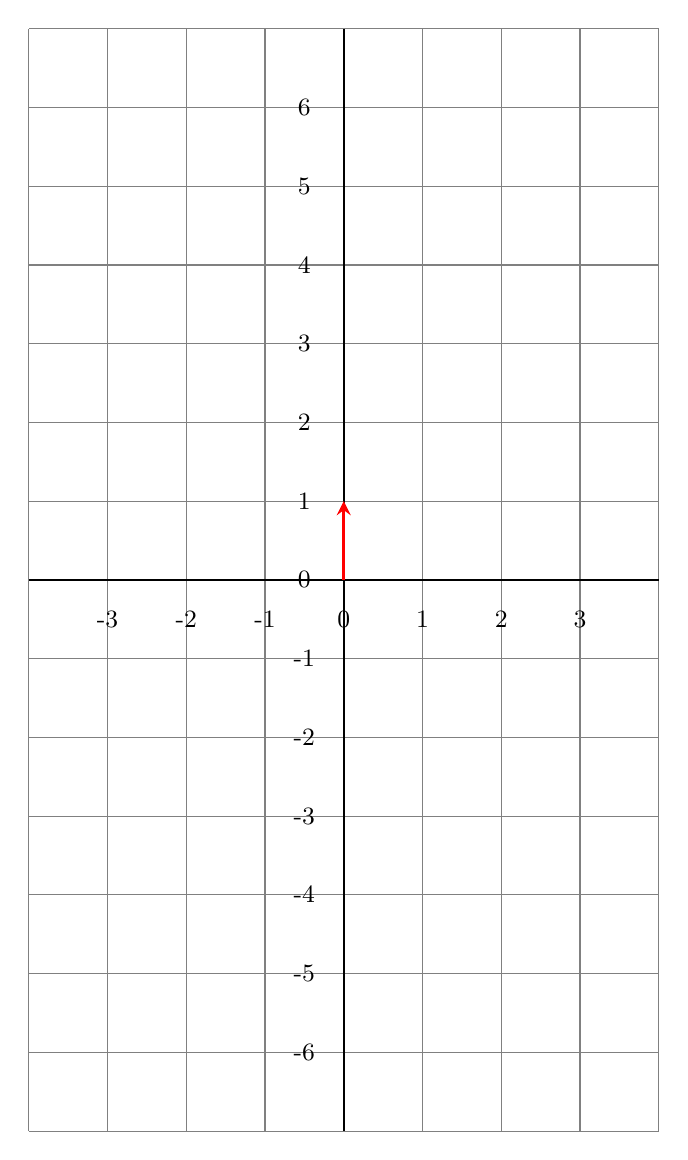
\begin{tikzpicture}
\draw[thin, step=1cm,color=gray] (-4,-7) grid (4,7);
\draw[thick] (-4,0)--(4,0);
\draw[thick] (0,7)--(0,-7);
\foreach \x in {-3,...,3}{
  \node at (\x,-0.5)  {\small{\x}};
}
\foreach \y in {-6,...,6}{
  \node at (-0.5,\y)  {\small{\y}};
}
\draw [very thick, red, -stealth] (0,0)--(0,1);
\end{tikzpicture}
\\
\end{tabular}
\newpage
Reflect the vector in the $x$-axis:
\newline
\newline
\begin{tabular}{p{13cm}p{13cm}}
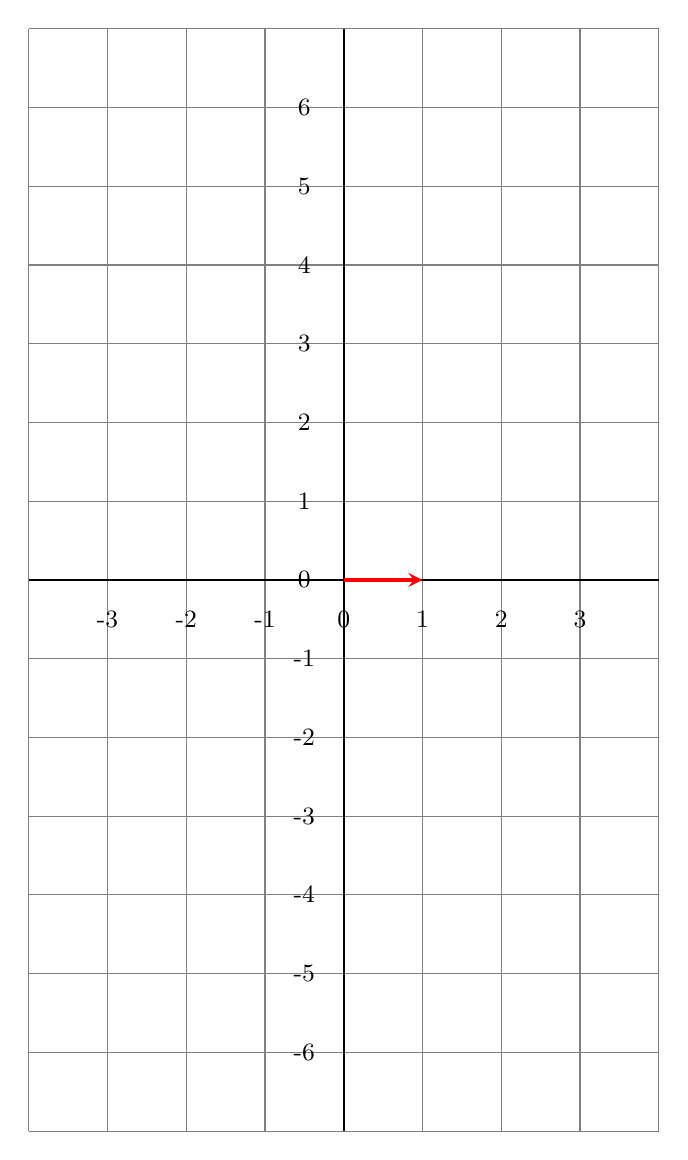
\begin{tikzpicture}
\draw[thin, step=1cm,color=gray] (-4,-7) grid (4,7);
\draw[thick] (-4,0)--(4,0);
\draw[thick] (0,7)--(0,-7);
\foreach \x in {-3,...,3}{
  \node at (\x,-0.5)  {\small{\x}};
}
\foreach \y in {-6,...,6}{
  \node at (-0.5,\y)  {\small{\y}};
}
\draw [very thick, red, -stealth] (0,0)--(1,0);
\end{tikzpicture}
&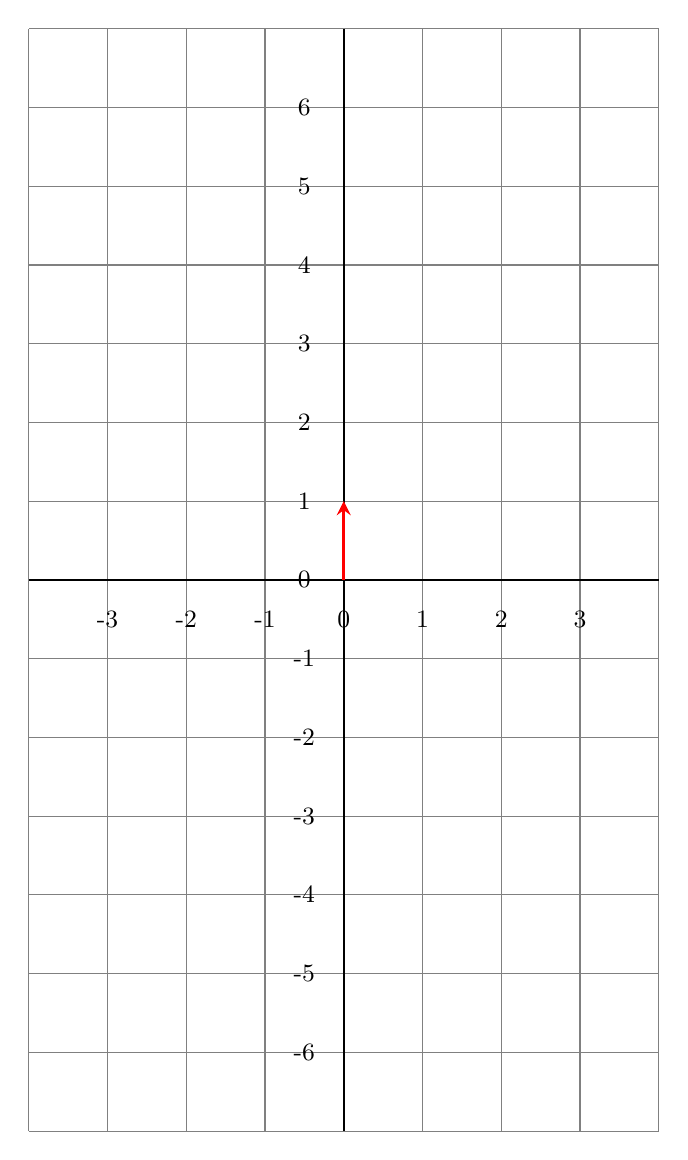
\begin{tikzpicture}
\draw[thin, step=1cm,color=gray] (-4,-7) grid (4,7);
\draw[thick] (-4,0)--(4,0);
\draw[thick] (0,7)--(0,-7);
\foreach \x in {-3,...,3}{
  \node at (\x,-0.5)  {\small{\x}};
}
\foreach \y in {-6,...,6}{
  \node at (-0.5,\y)  {\small{\y}};
}
\draw [very thick, red, -stealth] (0,0)--(0,1);
\end{tikzpicture}
\\
\end{tabular}
\newpage
Reflect the vector in the $y$-axis:
\newline
\newline
\begin{tabular}{p{13cm}p{13cm}}
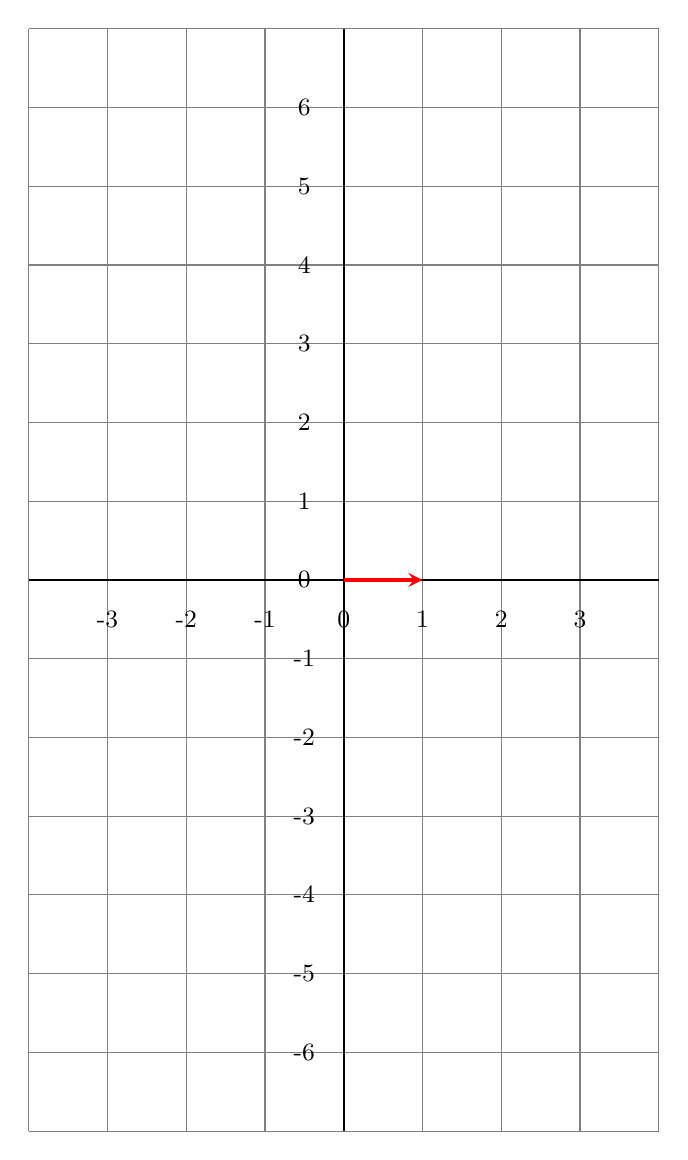
\begin{tikzpicture}
\draw[thin, step=1cm,color=gray] (-4,-7) grid (4,7);
\draw[thick] (-4,0)--(4,0);
\draw[thick] (0,7)--(0,-7);
\foreach \x in {-3,...,3}{
  \node at (\x,-0.5)  {\small{\x}};
}
\foreach \y in {-6,...,6}{
  \node at (-0.5,\y)  {\small{\y}};
}
\draw [very thick, red, -stealth] (0,0)--(1,0);
\end{tikzpicture}
&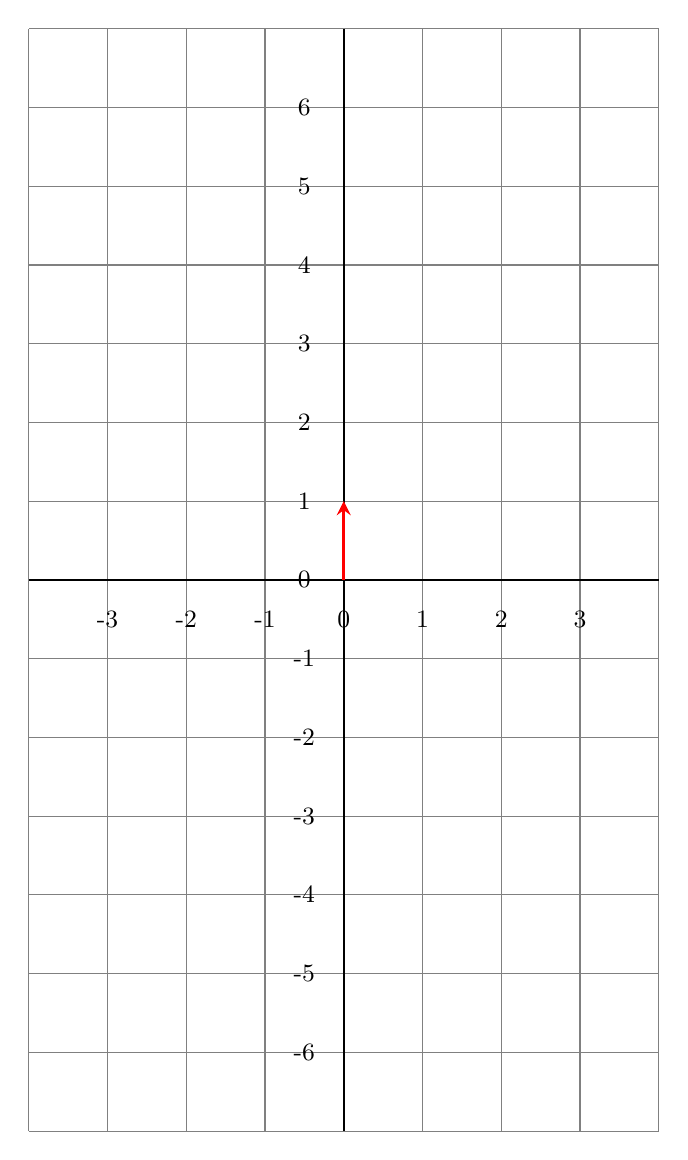
\begin{tikzpicture}
\draw[thin, step=1cm,color=gray] (-4,-7) grid (4,7);
\draw[thick] (-4,0)--(4,0);
\draw[thick] (0,7)--(0,-7);
\foreach \x in {-3,...,3}{
  \node at (\x,-0.5)  {\small{\x}};
}
\foreach \y in {-6,...,6}{
  \node at (-0.5,\y)  {\small{\y}};
}
\draw [very thick, red, -stealth] (0,0)--(0,1);
\end{tikzpicture}
\\
\end{tabular}
\newpage
Rotate the vector 90 degrees anti-clockwise:
\newline
\newline
\begin{tabular}{p{13cm}p{13cm}}
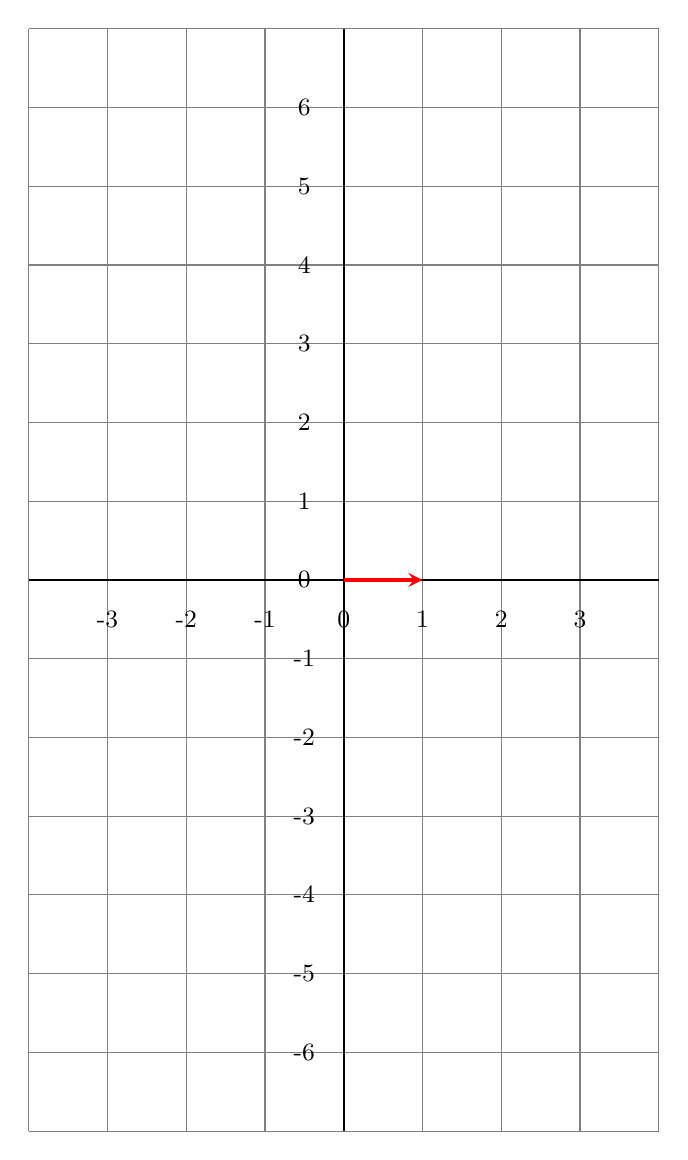
\begin{tikzpicture}
\draw[step=1cm,color=gray] (-4,-7) grid (4,7);
\draw[thick] (-4,0)--(4,0);
\draw[thick] (0,7)--(0,-7);
\foreach \x in {-3,...,3}{
  \node at (\x,-0.5)  {\small{\x}};
}
\foreach \y in {-6,...,6}{
  \node at (-0.5,\y)  {\small{\y}};
}
\draw [very thick, red, -stealth] (0,0)--(1,0);
\end{tikzpicture}
&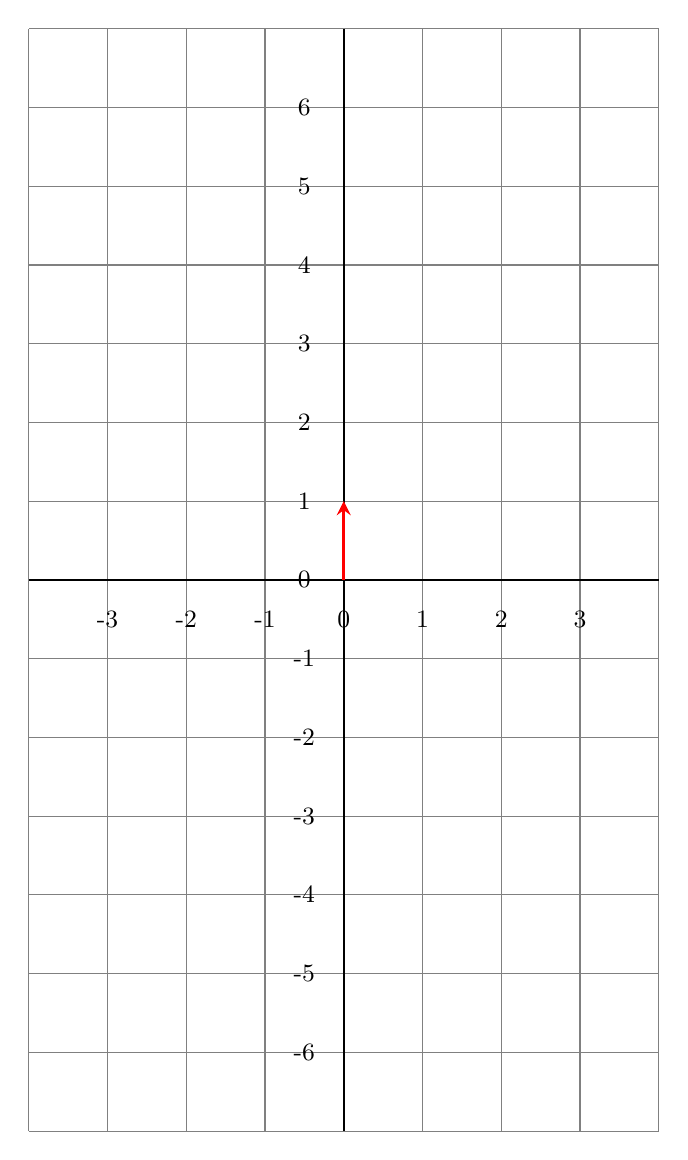
\begin{tikzpicture}
\draw[thin, step=1cm,color=gray] (-4,-7) grid (4,7);
\draw[thick] (-4,0)--(4,0);
\draw[thick] (0,7)--(0,-7);
\foreach \x in {-3,...,3}{
  \node at (\x,-0.5)  {\small{\x}};
}
\foreach \y in {-6,...,6}{
  \node at (-0.5,\y)  {\small{\y}};
}
\draw [very thick, red, -stealth] (0,0)--(0,1);
\end{tikzpicture}
\\
\end{tabular}
\newpage
Find a matrix which transforms the first vector into the second vector:
\newline
\newline
\begin{tabular}{p{13cm}p{13cm}}
$\begin{pmatrix}1\\0\end{pmatrix}, \begin{pmatrix}0\\1\end{pmatrix}$
&$\begin{pmatrix}1\\0\end{pmatrix}, \begin{pmatrix}1\\0\end{pmatrix}$
\\\\\\
\\\\\\

$\begin{pmatrix}1\\0\end{pmatrix}, \begin{pmatrix}-1\\0\end{pmatrix}$
&$\begin{pmatrix}1\\0\end{pmatrix}, \begin{pmatrix}0\\-1\end{pmatrix}$
\\\\\\
\\\\\\

$\begin{pmatrix}1\\0\end{pmatrix}, \begin{pmatrix}2\\0\end{pmatrix}$
&$\begin{pmatrix}1\\0\end{pmatrix}, \begin{pmatrix}0\\-2\end{pmatrix}$
\\\\\\
\end{tabular}
\newpage
Find a matrix which transforms the first vector into the second vector:
\newline
\newline
\begin{tabular}{p{13cm}p{13cm}}
$\begin{pmatrix}0\\1\end{pmatrix}, \begin{pmatrix}0\\1\end{pmatrix}$
&$\begin{pmatrix}0\\1\end{pmatrix}, \begin{pmatrix}1\\0\end{pmatrix}$
\\\\\\
\\\\\\

$\begin{pmatrix}0\\1\end{pmatrix}, \begin{pmatrix}-1\\0\end{pmatrix}$
&$\begin{pmatrix}0\\1\end{pmatrix}, \begin{pmatrix}0\\-1\end{pmatrix}$
\\\\\\
\\\\\\

$\begin{pmatrix}0\\1\end{pmatrix}, \begin{pmatrix}2\\0\end{pmatrix}$
&$\begin{pmatrix}0\\1\end{pmatrix}, \begin{pmatrix}0\\-2\end{pmatrix}$
\\\\\\
\end{tabular}
\newpage
Work out the matrix calculations
\newline
\newline
\begin{tabular}{p{13cm}p{13cm}}
$\begin{pmatrix}1&2\\3&4\end{pmatrix} \begin{pmatrix}5\\7\end{pmatrix}$
&$\begin{pmatrix}1&2\\3&4\end{pmatrix} \begin{pmatrix}6\\8\end{pmatrix}$
\\\\\\
\\\\\\

$\begin{pmatrix}1&2\\3&4\end{pmatrix} \begin{pmatrix}5&6\\7&8\end{pmatrix}$
&.
\\\\\\
\end{tabular}
\newpage
Work out the matrix calculations
\newline
\newline
\begin{tabular}{p{13cm}p{13cm}}
$\begin{pmatrix}1&2\\2&3\end{pmatrix} \begin{pmatrix}4\\7\end{pmatrix}$
&$\begin{pmatrix}1&2\\2&3\end{pmatrix} \begin{pmatrix}5\\8\end{pmatrix}$
\\\\\\
\\\\\\

$\begin{pmatrix}1&2\\2&3\end{pmatrix} \begin{pmatrix}4&5\\7&8\end{pmatrix}$
&.
\\\\\\
\end{tabular}
\newpage
Work out the transformation matrix for each transformation:
\newline
\newline
\begin{tabular}{p{13cm}p{13cm}}
Reflection in the line $y=x$
&Reflection in the $x$-axis
\\\\\\\\\\
\\\\\\\\\\

Reflection in the $y$-axis
&Reflection in the line $y=-x$
\\\\\\\\\\
\end{tabular}
\newpage
Work out the transformation matrix for each transformation:
\newline
\newline
\begin{tabular}{p{13cm}p{13cm}}
Enlargement by scale factor 2
&No change
\\\\\\\\\\
\\\\\\\\\\

Rotation 90 degrees anticlockwise about the origin
&Rotation 180 degrees about the origin
\\\\\\\\\\
\end{tabular}
\newpage
Work out the transformation matrix for each transformation:
\newline
\newline
\begin{tabular}{p{13cm}p{13cm}}
Rotation 90 degrees clockwise about the origin
&Rotation 45 degrees clockwise about the origin
\\\\\\\\\\
\\\\\\\\\\

Enlargement by scale factor -2
&Stretching by scale factor 2 along the x-axis
\\\\\\\\\\
\end{tabular}
\newpage
Work out the transformation matrix for a rotation of $\theta$ degrees anti-clockwise about the origin:
\newline
\newline
\begin{tabular}{p{13cm}p{13cm}}
\begin{tikzpicture}
\draw[step=2cm,color=gray] (-8,-6) grid (8,6);
\draw[thick] (-8,0)--(8,0);
\draw[thick] (0,6)--(0,-6);
\foreach \x in {-4,...,4}{
  \node at (\x*2,-0.5)  {\small{\x}};
}
\foreach \y in {-3,...,3}{
  \node at (-0.5,\y*2)  {\small{\y}};
}
\end{tikzpicture}
&
\end{tabular}
\end{document}
